% ==================================================================
%  Lessons 1 to 4: the theory on small examples, then the project's
%  reference choices.  Answers in answers_1_4.tex.
% ==================================================================

% ==================================================================
\section{One receiver: three directions the data cannot fix}\label{sec:l1}
% ==================================================================

\paragraph{Goal.} Start from the familiar user model and find the first null
directions: combinations of unknowns along which every observation stays the
same.

\paragraph{The idea.} For receiver $\rx$, satellite $\sat$ and signal $\sigl$ on
two frequencies, the code and phase equations of the status report (section
``One observation model'') are
\begin{align}
\code^\sat_{\rx,\sigl} &= \geomrange^\sat_\rx + \sLight(\mathrm{d}t_\rx - \mathrm{d}t^\sat)
  + T^\sat_\rx + \mu_\sigl I^\sat_\rx + B_{\rx,\sigl} - B^\sat_\sigl + \varepsilon,
  \label{eq:l1-code}\\
\phaseo^\sat_{\rx,\sigl} &= \geomrange^\sat_\rx + \sLight(\mathrm{d}t_\rx - \mathrm{d}t^\sat)
  + T^\sat_\rx - \mu_\sigl I^\sat_\rx + \lambda_\sigl N^\sat_{\rx,\sigl}
  + b_{\rx,\sigl} - b^\sat_\sigl + \varepsilon,
  \label{eq:l1-phase}
\end{align}
with $\mu_\sigl = f_1^2/f_\sigl^2$ (so $\mu_1 = 1$), $I^\sat_\rx$ the slant
ionospheric delay on the first frequency, $B$ and $b$ the code and phase biases,
and $N$ the ambiguity in cycles. A PPP user takes the orbit and the satellite
terms $\mathrm{d}t^\sat$, $B^\sat_\sigl$ and $b^\sat_\sigl$ from a product and
estimates the rest. Even then some combinations of the remaining unknowns leave
every observation unchanged. Such a combination is a null direction of the
design matrix: the data cannot fix a parameter along it, so a convention must.
The rest of the course follows these directions from one receiver into a
network.

\begin{question}{rx-clock}{derive}{The receiver clock and the code biases}{}
\begin{enumerate}[leftmargin=*, itemsep=1pt]
\item Show that the change $\sLight\,\mathrm{d}t_\rx \to \sLight\,\mathrm{d}t_\rx + \delta$,
      with every receiver bias $B_{\rx,1}, B_{\rx,2}, b_{\rx,1}, b_{\rx,2}$ changed
      by $-\delta$, leaves all four rows of a satellite unchanged.
\item Write the two receiver code biases as
      $B_{\rx,\sigl} = B_{\rx,\mathrm{IF}} + \mu_\sigl\, d_\rx$. Solve for
      $B_{\rx,\mathrm{IF}}$ and $d_\rx$ in terms of $B_{\rx,1}$ and $B_{\rx,2}$,
      and show that $B_{\rx,\mathrm{IF}}$ is their ionosphere-free combination.
\item Rewrite the code rows with this split. Which combination of clock and code
      biases do they contain, and what is a user's estimated ``receiver clock''
      therefore?
\end{enumerate}
\end{question}

\begin{question}{rx-phase}{derive}{The phase bias and the ambiguity}{\ref{q:rx-clock}}
\begin{enumerate}[leftmargin=*, itemsep=1pt]
\item Show that, for each signal $\sigl$, the change
      $b_{\rx,\sigl} \to b_{\rx,\sigl} - \delta_\sigl$ together with
      $N^\sat_{\rx,\sigl} \to N^\sat_{\rx,\sigl} + \delta_\sigl/\lambda_\sigl$ for
      every satellite leaves every phase row unchanged. How many such directions
      does one receiver have?
\item A PPP user estimates one float ambiguity per satellite and signal and no
      receiver phase bias. What does that float ambiguity contain, and why is it
      not an integer even with exact satellite phase biases?
\item What does a difference between two satellites at the same receiver
      remove, and what must the product supply for that difference to be an
      integer?
\end{enumerate}
\end{question}

\begin{question}{rx-iono}{derive}{The ionosphere and the geometry-free code bias}{\ref{q:rx-clock} and \ref{q:rx-phase}}
\begin{enumerate}[leftmargin=*, itemsep=1pt]
\item With the split of \cref{q:rx-clock}, show that the code rows of every
      satellite contain the slant ionosphere only as $I^\sat_\rx + d_\rx$.
\item Show that $I^\sat_\rx \to I^\sat_\rx + \delta$ for every satellite, with
      $d_\rx \to d_\rx - \delta$, leaves the code rows unchanged, and find what
      absorbs the change on the phase rows.
\item What does a user's estimated slant ionosphere therefore contain? What
      would have to be fixed by convention for it to be the physical ionosphere?
\end{enumerate}
\end{question}

\lessonbox{What this lesson establishes}{%
\begin{itemize}[leftmargin=*, itemsep=0pt, topsep=2pt]
\item One receiver has three kinds of null direction: the clock against the
      ionosphere-free code bias; each signal's phase bias against all of that
      signal's ambiguities; all slant ionospheres against the geometry-free code
      bias.
\item A parameter estimated along such a direction is a combination whose
      split a convention fixes: here the clock takes $B_{\rx,\mathrm{IF}}$, the
      ambiguities take the phase bias, the ionosphere takes $d_\rx$.
\item A network has the same directions at every receiver, and their mirror
      images at every satellite (\cref{sec:l2}). For the meeting: these
      directions are why a network must state its reference choices.
\end{itemize}}

% ==================================================================
\section{Two receivers: rank, reference choice and invariance}\label{sec:l2}
% ==================================================================

\paragraph{Goal.} Work the smallest network by hand: find its null directions,
remove them with a reference choice, and see what the choice changes and what it
cannot change.

\paragraph{The idea.} The Mathematical Reference works this example
(\texttt{docs/report/network\_example.tex}, ``Worked example: estimability in a
two-receiver network''). Receivers $A$ and $B$ observe satellites 1 to 4
(\cref{fig:l2-toy}). Positions are known; one frequency; no troposphere or
ionosphere; no noise. The code collapses to a difference of two clock lumps,
\begin{equation}
\code^\sat_\rx = a_\rx - g^\sat, \qquad
a_\rx = \sLight\,\mathrm{d}t_\rx + B_\rx, \qquad
g^\sat = \sLight\,\mathrm{d}t^\sat + B^\sat,
\label{eq:l2-code}
\end{equation}
which is the convention of \cref{q:rx-clock} already applied: each clock carries
its code bias. The phase is
\begin{equation}
\phaseo^\sat_\rx = a_\rx - g^\sat + b^\sat + N^\sat_\rx,
\label{eq:l2-phase}
\end{equation}
with $b^\sat$ the satellite phase bias and $N^\sat_\rx$ the ambiguity in metres,
which also absorbs the receiver's phase bias (\cref{q:rx-phase}). The truth, in
metres:
\begin{gather*}
a_A = 5,\quad a_B = 3;\qquad g = (2, -1, 4, 0.5);\qquad b = (0.10, -0.20, 0.05, 0.15);\\
N_A = (10, -5, 20, 8),\qquad N_B = (12, -3, 18, 9).
\end{gather*}
\begin{center}\small
\begin{tabular}{@{}lcccc@{\qquad}lcccc@{}}
\toprule
$\code^\sat_\rx$ & 1 & 2 & 3 & 4 & $\phaseo^\sat_\rx$ & 1 & 2 & 3 & 4 \\
\midrule
$A$ & 3 & 6 & 1 & 4.5 & $A$ & 13.10 & 0.80 & 21.05 & 12.65 \\
$B$ & 1 & 4 & $-1$ & 2.5 & $B$ & 13.10 & 0.80 & 17.05 & 11.65 \\
\bottomrule
\end{tabular}
\end{center}
A third receiver, $C$, appears in \cref{q:toy-user} as a user of the network's
corrections.

\begin{figure}[h]
\centering
\begin{tikzpicture}[
  sv/.style={draw, circle, fill=orange!15, minimum size=6.5mm, inner sep=0pt, font=\small},
  rcv/.style={draw, regular polygon, regular polygon sides=3, fill=blue!10,
              minimum size=9mm, inner sep=0pt, font=\small},
  usr/.style={draw, regular polygon, regular polygon sides=3, fill=green!12,
              minimum size=9mm, inner sep=0pt, font=\small}]
\foreach \i/\x in {1/0, 2/2.2, 3/4.4, 4/6.6} \node[sv] (s\i) at (\x, 3.1) {\i};
\node[rcv] (A) at (1.1, 0) {$A$};
\node[rcv] (B) at (3.8, 0) {$B$};
\node[usr] (C) at (6.6, 0) {$C$};
\foreach \i in {1, ..., 4} {
  \draw[gray!70] (A) -- (s\i);
  \draw[gray!70] (B) -- (s\i);
  \draw[green!50!black, dashed] (C) -- (s\i);}
\node[note, anchor=west] at (7.4, 3.1) {satellites 1 to 4};
\node[note, anchor=west] at (7.4, 0) {network: $A$, $B$;\ user: $C$};
\end{tikzpicture}
\caption{The worked example: two network receivers and four satellites; the user
$C$ of \cref{q:toy-user} applies the network's corrections.}
\label{fig:l2-toy}
\end{figure}

\begin{figure}[h]
\centering
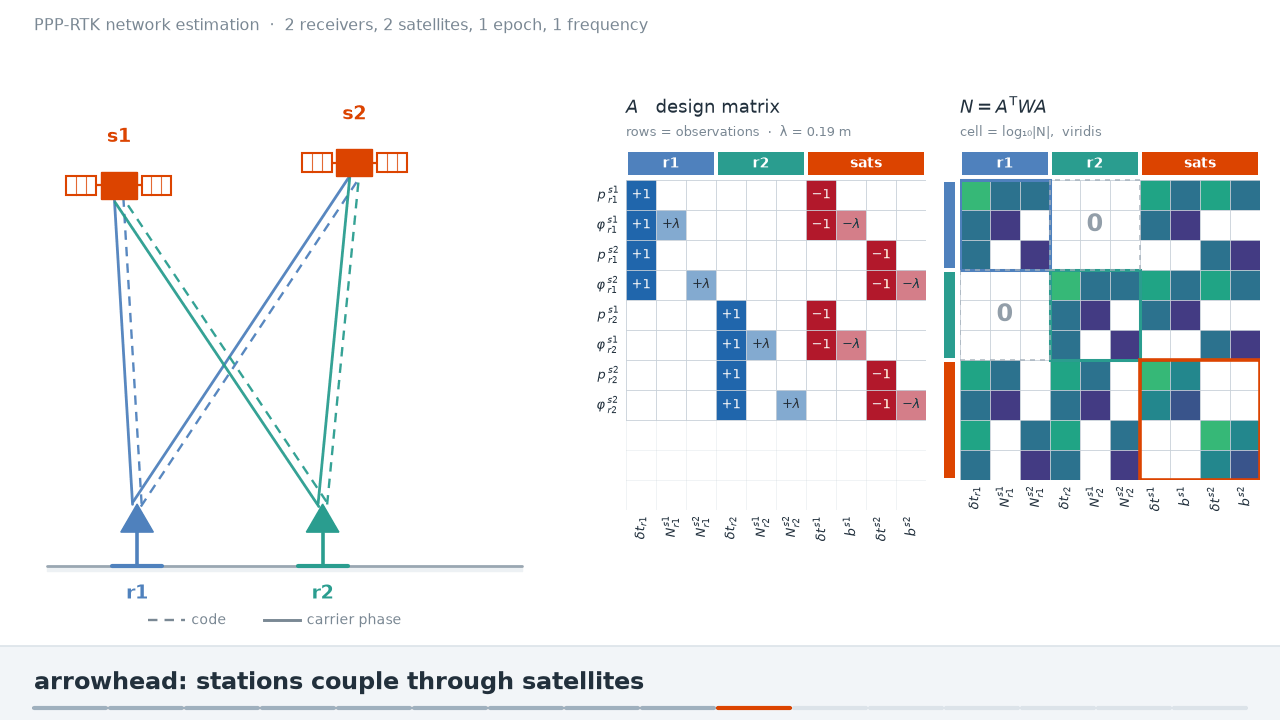
\includegraphics[width=0.49\linewidth]{toy_network_arrowhead.png}\hfill
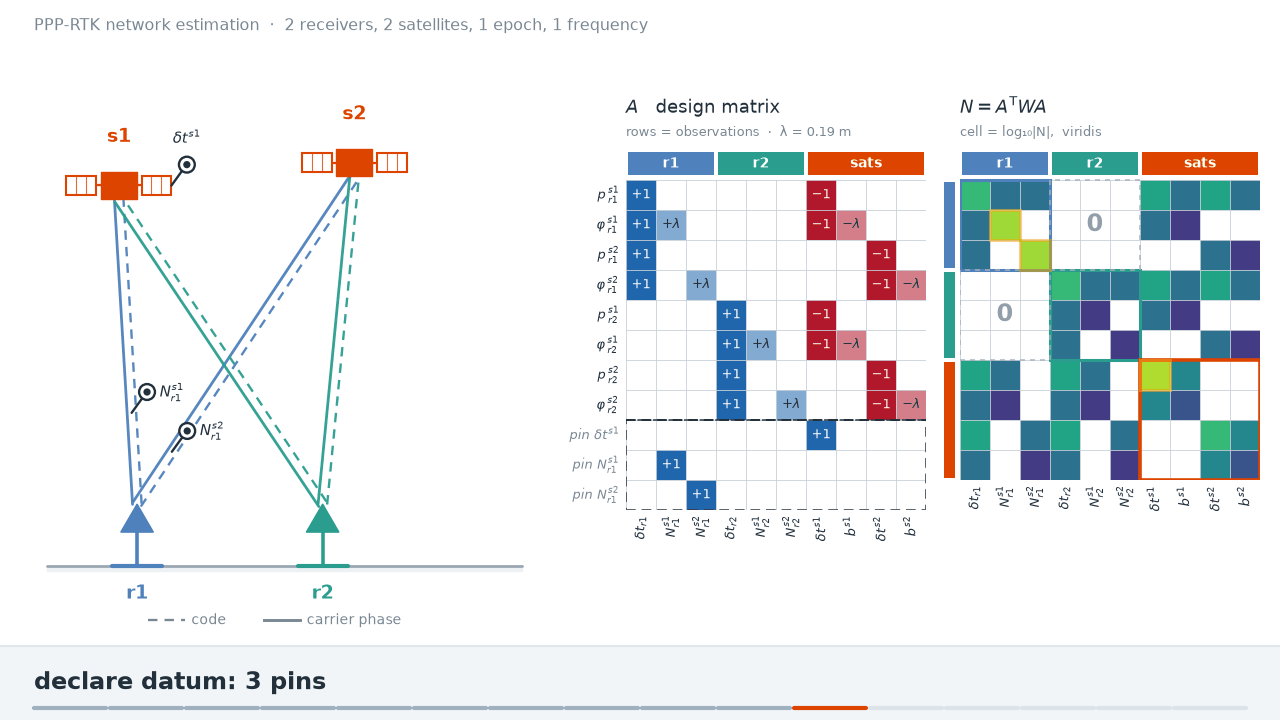
\includegraphics[width=0.49\linewidth]{toy_network_three_pins.png}
\caption{The same network with two satellites, from the project's concept
animation (\texttt{D:/GnssProcessorSupport/presentation/figures/network\_concept.gif}):
design matrix $\bm{A}$ and normal matrix $\bm{N} = \bm{A}^\Tr\bm{W}\bm{A}$. Left:
the empty blocks show that the receivers meet only through satellite terms.
Right: eight observations, ten unknowns, three null directions, removed by three
pins (the clock of satellite 1 and receiver $A$'s two ambiguities).}
\label{fig:l2-anim}
\end{figure}

\begin{question}{toy-normals}{derive}{The normal matrix and its null vector}{\ref{q:rx-clock}}
Order the unknowns $\bm{x} = [a_A, a_B, g^1, g^2, g^3, g^4]^\Tr$.
\begin{enumerate}[leftmargin=*, itemsep=1pt]
\item Write the $8\times6$ design matrix of the code rows and the normal matrix
      $\bm{N} = \bm{A}^\Tr\bm{A}$ (unit weights).
\item Show that $\bm{N}\bm{1} = \bm{0}$ for the all-ones vector. What is the rank
      of $\bm{N}$?
\item What change of the unknowns does $\bm{1}$ describe, and why can no number
      of observations of this kind fix it?
\end{enumerate}
\end{question}

\begin{question}{toy-datums}{derive}{Two reference choices, one fit}{\ref{q:toy-normals}}
\begin{enumerate}[leftmargin=*, itemsep=1pt]
\item Solve the code rows with the pin $a_A \equiv 0$, then with the pin
      $g^1 \equiv 0$.
\item Subtract the two solutions. What is the difference, in the terms of
      \cref{q:toy-normals}?
\item Compute $a_A - a_B$, $g^2 - g^1$, $g^3 - g^1$ and $a_B - g^4$ in both
      solutions. Why do they agree?
\item Under $a_A \equiv 0$, what does the estimated clock of satellite 2 equal in
      terms of the true clocks?
\end{enumerate}
\end{question}

\begin{question}{toy-phase}{derive}{Phase: the satellite phase bias needs a second receiver}{\ref{q:toy-datums}}
\begin{enumerate}[leftmargin=*, itemsep=1pt]
\item With code and phase together, count the unknowns, the observations, the
      null directions and the redundancy. Which null directions does the phase
      add?
\item With receiver $A$ alone, what does each satellite's phase determine, and
      which pair of unknowns can it not separate? What changes with receiver $B$?
\item Apply the reference choice $a_A \equiv 0$ with $N^\sat_A \equiv 0$ for every
      satellite. Compute the emitted phase bias $\bar b^\sat$ and the estimate
      $\hat N^\sat_B$ for the four satellites.
\item The physical phase bias of satellite 1 is 0.10~m and the emitted one
      10.10~m. What did it absorb? What is $\hat N^\sat_B$?
\end{enumerate}
\end{question}

\begin{question}{toy-biases}{derive}{Where the hardware biases went}{\ref{q:rx-clock}, \ref{q:rx-phase} and \ref{q:toy-phase}}
Write the network with every hardware bias explicit: receiver and satellite code
biases $B_\rx$, $B^\sat$, receiver and satellite phase biases $b_\rx$, $b^\sat$,
and the integer ambiguities. For $f$ frequencies, $n$ receivers and $m$
satellites, Odijk et al.~\cite{odijk2016estimability} count six types of null
direction (\texttt{SBASIS-THEORY-E.md}, section E2): 1a, receiver clock against
satellite clock, 1; 1b, receiver against satellite hardware biases, $2f$; 2a,
receiver clock against receiver biases, $n-1$; 3a, satellite clock against
satellite biases, $m$; 4, receiver phase bias against ambiguities, $f(n-1)$; 5,
satellite phase bias against ambiguities, $f\,m$.
\begin{enumerate}[leftmargin=*, itemsep=1pt]
\item Evaluate the six types for $f = 1$, $n = 2$, $m = 4$ and add them.
\item The worked example defined $a_\rx$, $g^\sat$ and $N^\sat_\rx$ as lumps.
      How many unknowns did the lumps remove, and how does the rank change?
      Which types are gone and which remain? Check the remainder against
      \cref{q:toy-phase}.
\end{enumerate}
\end{question}

\begin{question}{toy-user}{derive}{A user of the emitted corrections}{\ref{q:toy-datums} and \ref{q:toy-phase}}
A third receiver $C$, not in the network, has the truth $a_C = 4$ and
$N_C = (11, -4, 19, 10)$~m.
\begin{enumerate}[leftmargin=*, itemsep=1pt]
\item Compute its four code and four phase observations.
\item $C$ applies the network's satellite clocks $\hat g^\sat$ (from the choice
      $a_A \equiv 0$) and phase biases $\bar b^\sat$. Solve for its clock
      $\hat a_C$ and its ambiguities $\tilde N^\sat_C$.
\item What do $\hat a_C$ and $\tilde N^\sat_C$ equal in terms of the true values?
      Whose values does $C$'s solution carry, and does $C$ need to know it?
\end{enumerate}
\end{question}

\begin{question}{toy-setchange}{derive}{When the satellite set changes}{\ref{q:toy-datums}}
\begin{enumerate}[leftmargin=*, itemsep=1pt]
\item From the solution with $g^1 \equiv 0$, give the solution under the
      sum-to-zero choice $\sum_\sat g^\sat = 0$ over the four satellites.
\item Satellite 4 sets. Recompute both solutions with satellites 1 to 3. By how
      much does every clock move under each choice?
\item Instead satellite 1, the pinned one, sets, and the pin moves to satellite
      2. By how much does every clock move?
\item Does any of these changes move an estimable quantity? What must a user be
      told at such an epoch, and why?
\end{enumerate}
\end{question}

\lessonbox{What this lesson establishes}{%
\begin{itemize}[leftmargin=*, itemsep=0pt, topsep=2pt]
\item A reference choice is a set of pins or rows that removes the null
      directions; every admissible choice fits the data equally well.
\item Differences (estimable functions) agree under every choice; the emitted
      values carry the choice (the satellite clock carries the reference
      receiver's clock, the phase bias its ambiguity).
\item A user applying the corrections inherits the network's reference without
      knowing it: its estimates are relative to the network.
\item A sum-to-zero reference moves whenever a satellite rises or sets; a pin
      moves only when its own satellite leaves. Either move must be declared.
\end{itemize}}

% ==================================================================
\section{The real network: elimination, counting and the rank gate}\label{sec:l3}
% ==================================================================

\paragraph{Goal.} Scale the worked example up to the real network: eliminate the
stations, count the null directions, and find them again in a run.

\paragraph{The idea.} The network processor solves one joint system per epoch
over all stations (status report, step 6). The unknowns shared by all stations,
$\bm{x}_{\mathrm{B}}$, are the satellite clocks, code biases and phase biases;
each station $\rx$ has its own, $\bm{x}_\rx$: ambiguities, slant ionosphere,
zenith wet delay, receiver clock, inter-system bias and receiver code-bias
difference. Stations meet only through $\bm{x}_{\mathrm{B}}$, so the normal
matrix is an arrowhead (\cref{fig:l2-anim}, left) and each station's block is
eliminated exactly before the shared solve:
\begin{equation}
\bar{\bm{N}}_{\mathrm{BB}} = \sum_{\rx}\Big(\bm{N}^{(\rx)}_{\mathrm{BB}}
  - \bm{N}_{\mathrm{B}\rx}\bm{N}_{\rx\rx}^{-1}\bm{N}_{\mathrm{B}\rx}^\Tr\Big)
  + \bm{N}^{\mathrm{prior}}_{\mathrm{BB}},
\qquad
\bm{x}_\rx = \bm{N}_{\rx\rx}^{-1}\big(\bm{u}_\rx - \bm{N}_{\mathrm{B}\rx}^\Tr\bm{x}_{\mathrm{B}}\big).
\label{eq:l3-schur}
\end{equation}
From epoch to epoch the solution is a Kalman filter in information form. Every
epoch a check, the \emph{rank gate}, counts the eigenvalues of
$\bar{\bm{N}}_{\mathrm{BB}}$ below $\mathtt{rank\_gate\_tol}\times\lambda_{\max}$
and requires exactly the declared number (\texttt{include/network/solve/Sbasis.hpp},
\texttt{src/core/network/solve/RankGate.cpp}). A single-receiver PPP filter has
the same shape, with epochs in the place of stations (\cref{fig:l3-ppp}).

\begin{figure}[h]
\centering
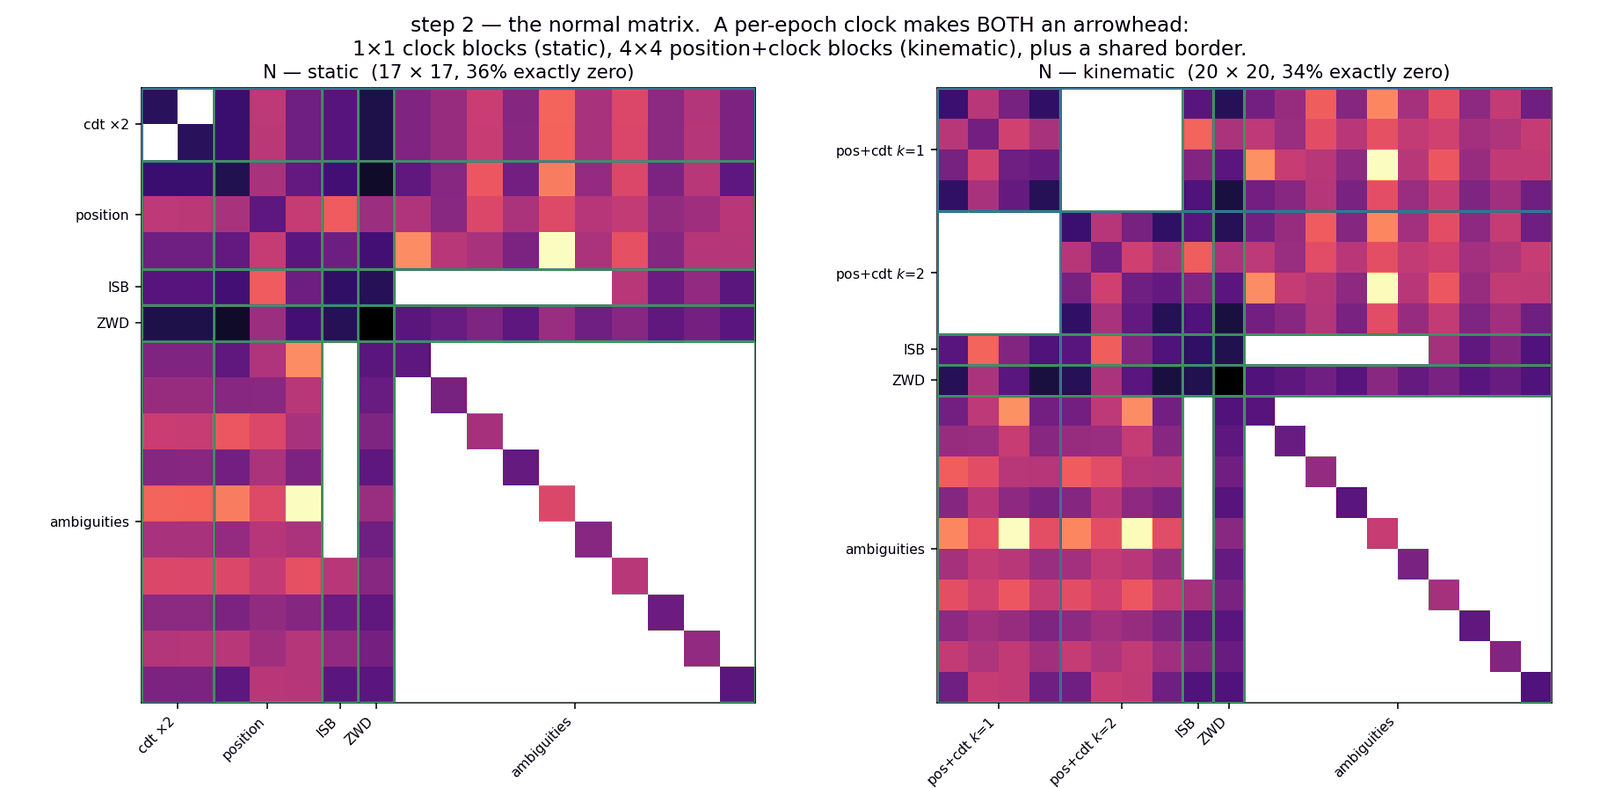
\includegraphics[width=0.62\linewidth]{per_epoch_arrowhead.png}\hfill
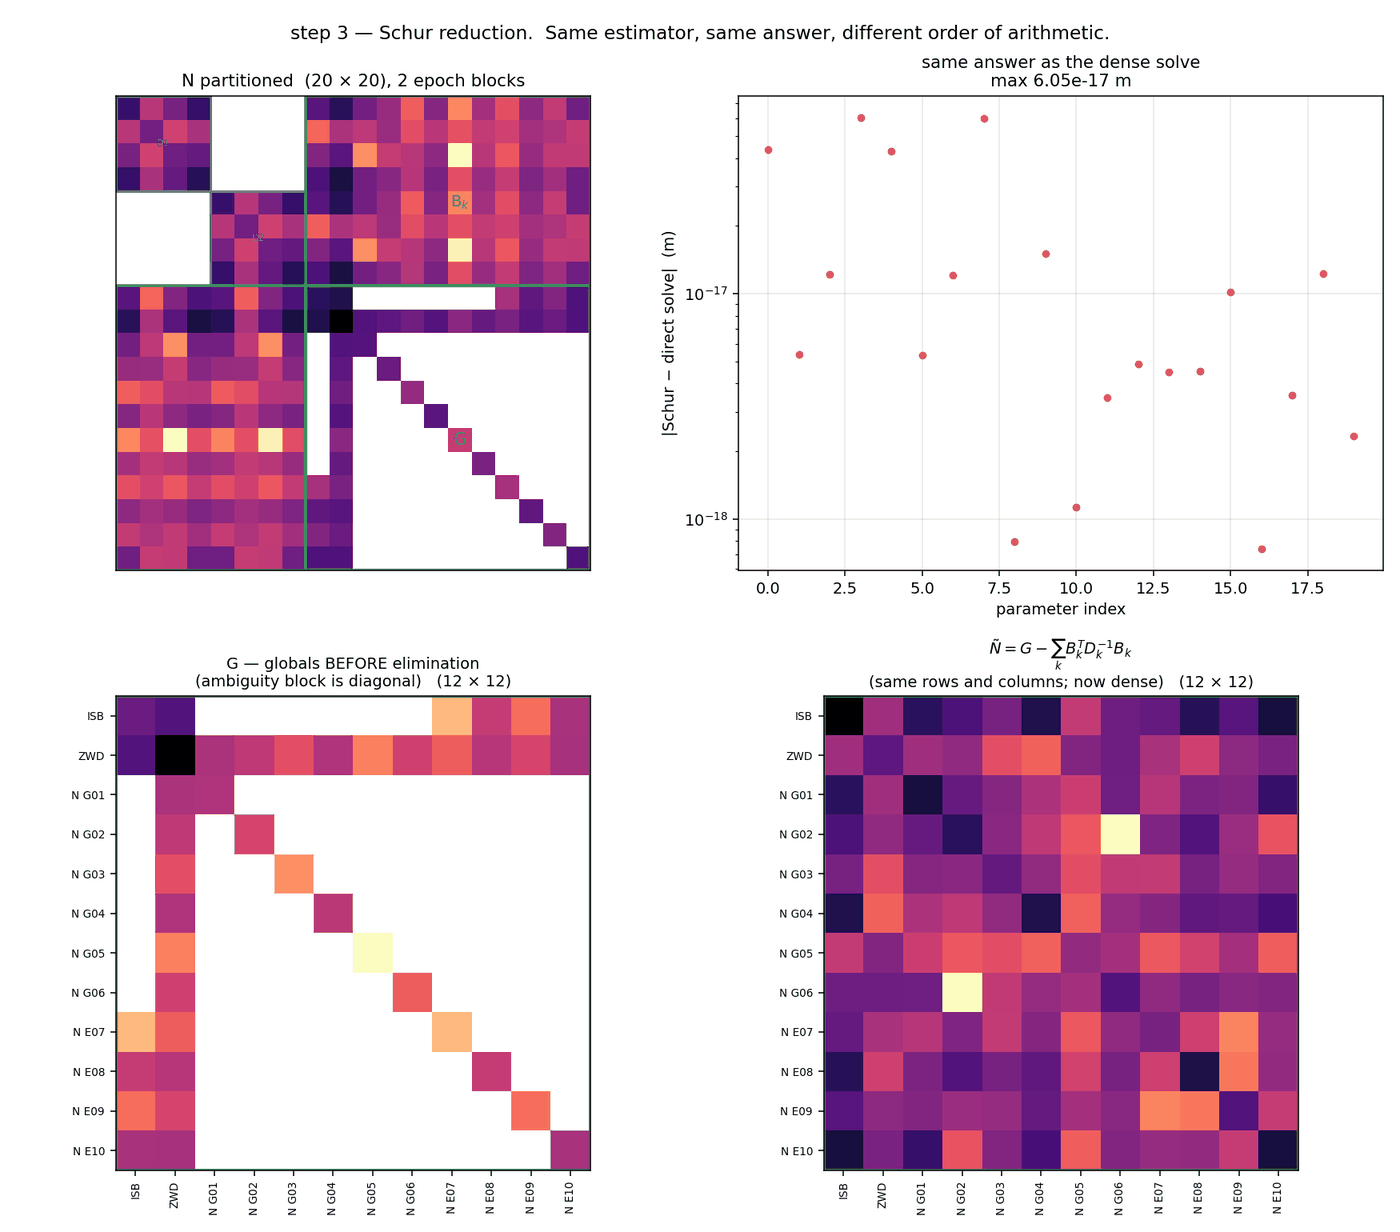
\includegraphics[width=0.36\linewidth]{schur_equals_direct.png}
\caption{Left: one receiver over two epochs; a clock per epoch makes $1\times1$
(static) or $4\times4$ (moving receiver) epoch blocks around a shared border.
Right: eliminating the blocks first gives the direct solution to $6\times10^{-17}$~m.
September 2026 illustrations.}
\label{fig:l3-ppp}
\end{figure}

\begin{question}{schur}{derive}{Eliminating the receivers}{\ref{q:toy-normals} and \ref{q:toy-datums}}
In the code system of \cref{q:toy-normals}, the receiver clocks are the local
unknowns and the satellite clocks the shared ones.
\begin{enumerate}[leftmargin=*, itemsep=1pt]
\item Compute the reduced shared normal
      $\bar{\bm{N}}_{gg} = \bm{N}_{gg} - \bm{N}_{ga}\bm{N}_{aa}^{-1}\bm{N}_{ag}$ and
      the reduced right-hand side
      $\bar{\bm{u}}_g = \bm{u}_g - \bm{N}_{ga}\bm{N}_{aa}^{-1}\bm{u}_a$ from the
      pseudorange table.
\item Find the eigenvalues of $\bar{\bm{N}}_{gg}$ and its normalized null
      eigenvector. What weight does it put on each satellite clock?
\item Solve the reduced system with $g^1 \equiv 0$, then back-substitute the
      receiver clocks with \cref{eq:l3-schur}. Compare with \cref{q:toy-datums}.
\end{enumerate}
\end{question}

\begin{question}{twosys}{derive}{Two constellations}{\ref{q:schur}}
Add Galileo satellites. Each receiver gets an inter-system bias $d^{E}_\rx$ on its
Galileo rows ($d^{G}_\rx \equiv 0$ by definition: GPS is the reference system), so
$\code^\sat_\rx = a_\rx + d^{g(\sat)}_\rx - g^\sat$.
\begin{enumerate}[leftmargin=*, itemsep=1pt]
\item Find the null directions of this system.
\item After the receiver clocks and inter-system biases are eliminated, how many
      null directions does the reduced shared normal keep, and what do they look
      like on the satellite clocks?
\item For 32 GPS and 24 Galileo satellites, what weight does each normalized
      direction put on each clock?
\end{enumerate}
\end{question}

\begin{question}{eq24}{derive}{Eq.~24 for the real network}{\ref{q:rx-iono} and \ref{q:toy-biases}}
\begin{enumerate}[leftmargin=*, itemsep=1pt]
\item Sum the six types of \cref{q:toy-biases} to obtain Eq.~24 of
      \cite{odijk2016estimability}, $1 + 2f + (1+f)(n-1+m)$. Add the
      slant-ionosphere term $n - 1 + m$ (the direction of \cref{q:rx-iono}, now at
      every receiver and every satellite).
\item \Cref{fig:l3-count} uses one constellation of 32 satellites and two
      frequencies with a slant ionosphere. Check its 369 directions for 60
      stations, 361 for 58 and 1,349 for 305.
\item The first epoch of the simulated reference run has $n = 60$, $m = 56$ (32
      GPS, 24 Galileo) and $f = 2$. What does Eq.~24 with the slant term give?
\end{enumerate}
\end{question}

\begin{figure}[h]
\centering
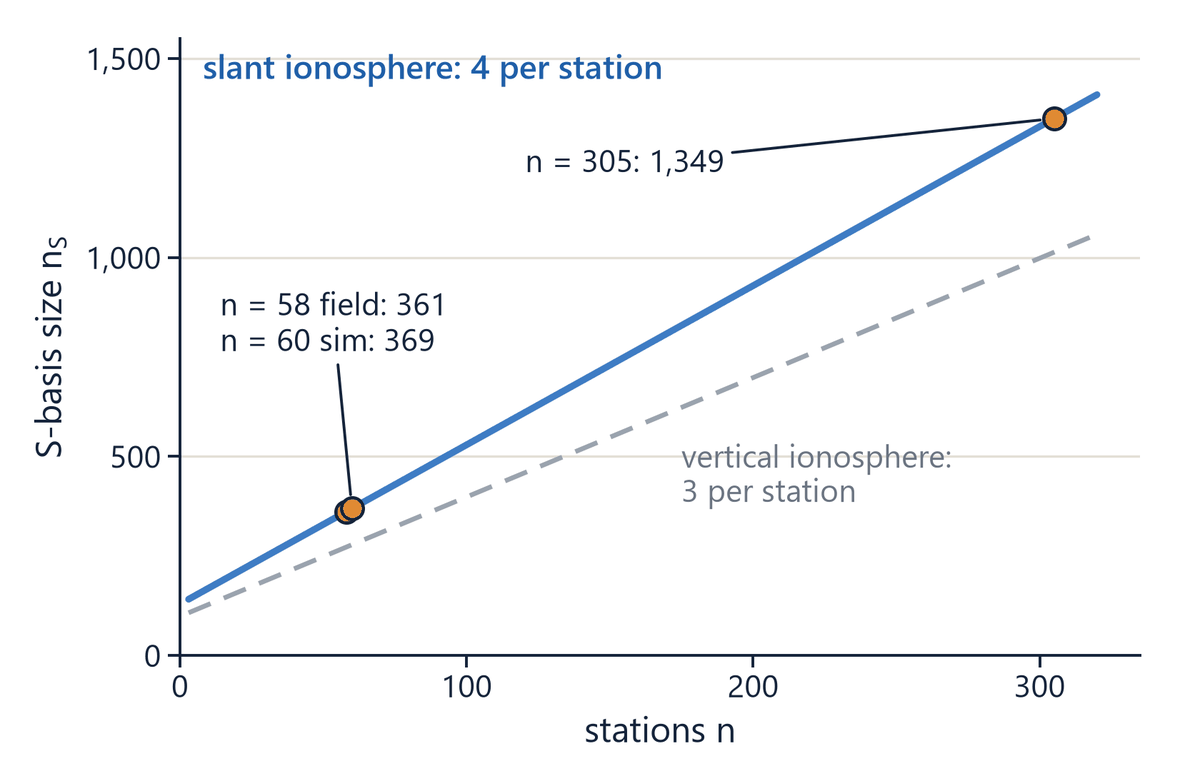
\includegraphics[width=0.48\linewidth]{undetermined_directions.png}\hfill
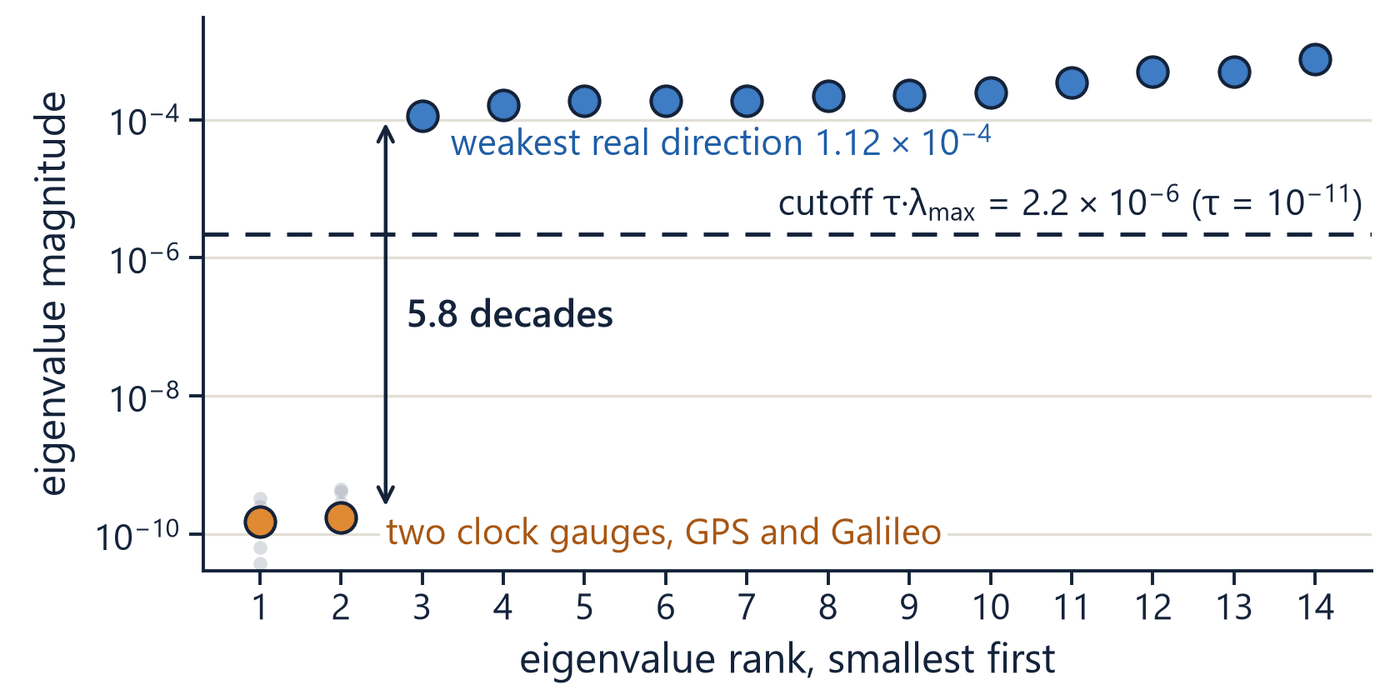
\includegraphics[width=0.5\linewidth]{rank_gate_eigenvalues.png}
\caption{Left: Eq.~24 against the number of stations, one constellation of 32
satellites, two frequencies: about four more directions per station with a slant
ionosphere, three with a vertical one (deck slide 6). Right: the rank gate on the
first real-data epoch, the 14 smallest eigenvalues of the $414\times414$ reduced
shared normal matrix: two near $10^{-10}$ (one clock direction per constellation),
the weakest real direction 5.8 decades higher, the dashed line the cutoff (deck
slide 7).}
\label{fig:l3-count}
\end{figure}

\begin{question}{inventory}{read}{The parameters as armed}{\ref{q:rx-clock} to \ref{q:rx-iono} and \ref{q:schur}}
Print the table of the simulated reference run (60 stations, GPS and Galileo,
two signals each):
\begin{cmd}
sed -n '658,686p' runs/_rf0hv15_sim6/stdout.txt
\end{cmd}
\begin{enumerate}[leftmargin=*, itemsep=1pt]
\item Map each unknown of \cref{eq:l1-code,eq:l1-phase} to a row of the table.
      Which term has no row, and where did \cref{q:rx-phase} put it?
\item How many shared and how many local columns does the run carry at its first
      epoch?
\end{enumerate}
\end{question}

\begin{question}{rankgate}{measure}{The rank gate on the real network}{\ref{q:twosys} and \ref{q:eq24}}
Run (about 9~s):
\begin{cmd}
C:/Python313/python.exe -I scripts/rf_null_space_read.py runs/_rf0hv15_sim6
grep -n "rank gate evaluated" runs/_rf0hv15_sim6/stdout.txt
\end{cmd}
\begin{enumerate}[leftmargin=*, itemsep=1pt]
\item Which two eigenvalues fall below the cutoff at the first epoch, and what
      weights do their eigenvectors carry? Compare with \cref{q:twosys}.
\item How many decades lie between the cutoff and the larger of the two, and
      between the cutoff and the weakest real direction? Does that meet the
      placement rule of \texttt{src/core/network/solve/RankGate.cpp} (lines 408
      to 410)?
\item Eq.~24 gave 465 directions; the gate declares 2. Where did the others go?
      (\Cref{q:toy-biases} holds the key; \cref{q:rows} counts the rows.)
\end{enumerate}
\end{question}

\lessonbox{What this lesson establishes}{%
\begin{itemize}[leftmargin=*, itemsep=0pt, topsep=2pt]
\item Eliminating the stations is exact; the reduced shared normal keeps the
      network's shared null directions.
\item With two constellations the shared null space is two flat clock shifts,
      weight $1/\sqrt{m_g}$ on every clock of system $g$; the real run shows
      exactly these, at 0.1767 and 0.2040.
\item Eq.~24 counts hundreds of directions; lumps, pins and priors remove almost
      all of them before the gate, which sees one per constellation. For the
      meeting: the per-epoch check confirms this count on every epoch.
\end{itemize}}

% ==================================================================
\section{The project's four reference choices}\label{sec:l4}
% ==================================================================

\paragraph{Goal.} Name the reference choices the reference configurations make,
count their rows, and find the one direction they leave to a weak prior.

\paragraph{The idea.} A reference choice is a set of constraints
$\bm{B}^\Tr\bm{x} = \bm{0}$, or pins, that picks one solution among those that fit
the data equally well. The S-transformation
$\bm{S} = \bm{I} - \bm{V}[(\bm{S}^\perp)^\Tr\bm{V}]^{-1}(\bm{S}^\perp)^\Tr$ projects
onto the estimable space along the null space $\bm{V}$; its rows are the
estimable combinations, and the reference directions carry zero variance
(\texttt{SBASIS-THEORY-E.md}, section E1, after \cite{teunissen1985generalised,
odijk2016estimability}). The record names four kinds of choice (section E3), each
with an analogue in \cref{sec:l2}: a \emph{pin} ($g^1 \equiv 0$); a
\emph{prioritized anchor} ($N^\sat_A \equiv 0$, but elected per satellite and
signal); a \emph{sum-to-zero} row ($\sum g^\sat = 0$); an \emph{ensemble}, an inner
constraint over all receivers, measured dead and deleted on 2026-10-14. The
reference configurations combine four choices:

\begin{center}\footnotesize
\begin{tabular}{@{}p{2.6cm}p{4.1cm}p{4.6cm}p{2.9cm}@{}}
\toprule
Choice & What it fixes & Settings (\texttt{golden\_sim\_refound.json}) & First epoch, simulated \\
\midrule
Clock pin & one satellite clock per constellation (the pivot); \cref{q:toy-datums,q:twosys} & no key (the default); \texttt{sticky\_pivot}, \texttt{handover\_stransform} & 2 pins (E02, G01) \\
Prioritized phase anchors, held basis & one ambiguity per satellite and signal, frozen at its basis value; \cref{q:toy-phase} & \texttt{phase\_datum\_prioritized}, \texttt{phase\_datum\_held\_basis}, \texttt{ambiguity\_vehicle} \texttt{float\_kf} & 112 pins on 18 stations \\
Code-bias datum & per satellite the ionosphere-free pin and the geometry-free pin at the broadcast $T_{GD}$; \cref{q:rx-clock,q:rx-iono} at the satellites & \texttt{estimate\_sat\_code\_bias}, \texttt{sat\_gf\_datum} \texttt{broadcast\_tgd}, \texttt{sat\_gf\_datum\_time\_linked} & $56 + 56$ rows \\
Zero-mean receiver DCB prior & the mean of the receivers' geometry-free code biases, $\sigma$ 10~m; \cref{q:rx-iono} at the receivers & \texttt{rx\_code\_bias\_datum}, \texttt{station\_prior\_before\_pd} & 120 prior entries on 60 stations \\
\bottomrule
\end{tabular}
\end{center}

One direction per station and constellation is left to the weak prior: the
station's \emph{level}, its slant ionosphere, receiver geometry-free code biases
and ambiguities shifted together. It is local, so it is eliminated before the
rank gate sees anything.

\begin{question}{theorem}{read}{The theorem in the record}{\ref{q:toy-datums}}
Read the boxed theorem of \texttt{SBASIS-THEORY-E.md}, section E1, and the
paragraph ``Datum-invariant even before choosing a datum'' of section E2.
\begin{enumerate}[leftmargin=*, itemsep=1pt]
\item What exactly is invariant, and under which choices? Where did
      \cref{q:toy-datums} show it in six unknowns?
\item Which of these are estimable before any choice: position, zenith delay,
      vertical ionosphere, a satellite clock, a satellite phase bias?
\item A differential satellite clock wander of about 47~cm was measured before
      the re-founding. Why could no change of reference cure it, and what kind of
      change can?
\end{enumerate}
\end{question}

\begin{question}{four}{read}{Four choices in the reference configuration}{\ref{q:toy-phase}, \ref{q:toy-setchange} and \ref{q:theorem}}
Confirm that the reference configurations are the generated ones, then read
\texttt{config/golden/golden\_sim\_refound.json}:
\begin{cmd}
C:/Python313/python.exe scripts/make_golden_config.py --verify
\end{cmd}
\begin{enumerate}[leftmargin=*, itemsep=1pt]
\item Through which keys does the file arm each choice of the table above?
\item How does each choice behave when a satellite rises or sets, and which of
      them, by \cref{q:toy-setchange}, would move at every rise and set?
\item Which datum-looking keys are absent from the file?
\end{enumerate}
\end{question}

\begin{question}{rows}{derive}{The rows of the first epoch}{\ref{q:rankgate} and \ref{q:four}}
The simulated case's first epoch has 56 satellites (32 GPS, 24 Galileo) at 60
stations, two signals per constellation; each satellite carries one clock, two
phase biases and two code biases.
\begin{enumerate}[leftmargin=*, itemsep=1pt]
\item How many shared columns are there, and how many rows does each choice
      contribute?
\item Account for the gate's 2: which rows act before the gate, and which after?
\item What does the solver do on an epoch whose count differs, and what would
      S-basis completion add?
\end{enumerate}
Check against lines 631, 679 to 738 and 4109 to 4112 of
\texttt{D:/GnssProcessorSupport/runs\_nom/\_rap\_scb\_g\_q6/stdout.txt}.
\end{question}

\begin{question}{cbdatum}{measure}{The code-bias datum on the corrections}{\ref{q:rx-clock} and \ref{q:rx-iono}}
Read the first epoch's code-bias records of G05 in the simulated reference case
and the G05 record of the broadcast navigation file:
\begin{cmd}
grep -n -m2 '^B,G05,' D:/GnssProcessorSupport/runs_nom/_rap_scb_g_q6/products.txt
sed -n '562,568p' data/2024-129/products/BRDC00IGS_R_20241290000_01D_MN.rnx
\end{cmd}
\begin{enumerate}[leftmargin=*, itemsep=1pt]
\item What is the ratio of the C2W record to the C1C record, what is their
      ionosphere-free combination, and how does the C1C record compare with
      $c\,T_{GD}$?
\item Where does the satellite's true geometry-free code bias go in the network
      solution, and what must a user do with its own slant ionosphere for the
      records to apply?
\end{enumerate}
\end{question}

\begin{question}{level}{derive}{The direction the shared check cannot see}{\ref{q:rx-iono}, \ref{q:schur} and \ref{q:rows}}
Card R1D (section 1) gives the loadings of the GPS level direction of station
MAJU00MHL: the receiver DCB carries a share 0.0074 of the unit direction, the
band-5 code delay $0.2392^2$ and the second-channel offset $0.1334^2$. The
receiver DCB prior has $\sigma = 10$~m.
\begin{enumerate}[leftmargin=*, itemsep=1pt]
\item What standard deviation does the prior alone give along the unit level
      direction? Check the card's ``about 116~m''.
\item A zero-mean row on the band-5 delay and the second-channel offset at the
      same $\sigma$ would add information. By what factor? Check ``about eleven
      times''.
\item Card ALD (section 3) gives $v^\Tr N v = 110$ per unit level for the coupling
      rows. What $\sigma$ follows, and which rows hold the level?
\item Why can the rank gate never see this direction, and how did it carry the
      GPS L5 event into the corrections?
\end{enumerate}
\end{question}

\lessonbox{What this lesson establishes}{%
\begin{itemize}[leftmargin=*, itemsep=0pt, topsep=2pt]
\item No admissible reference choice changes an estimable value or its variance;
      only estimation (weights, dynamics, model) can.
\item The project pins one clock per constellation, anchors one ambiguity per
      satellite and signal, pins each satellite's code biases to the broadcast
      group delay, and holds the receivers' code-bias mean with a weak prior.
\item The published code biases of the pinned pair carry no estimate; the
      ionosphere absorbs the true geometry-free bias.
\item Each station's level is held by the carried coupling, not by the datum,
      and the gate cannot see it. For the meeting: the choices are 226 rows and
      120 prior entries at the first simulated epoch, not ``a few''.
\end{itemize}}
